% Flip-Chip Cross-Section: Face-Down Die on Interposer
\documentclass[border=3mm]{standalone}
\usepackage{tikz}
\usetikzlibrary{arrows.meta, positioning, calc, decorations.pathreplacing}
\usepackage[T1]{fontenc}
\usepackage{lmodern}

% IHP Colors
\definecolor{IHPfg}{RGB}{0,80,139}
\definecolor{IHPaccent}{RGB}{109,112,114}
\definecolor{IHPgreen}{RGB}{65,155,75}
\definecolor{cInterposer}{RGB}{0,80,139}
\definecolor{cDie}{RGB}{55,145,195}
\definecolor{cCuPillar}{RGB}{184,115,51}
\definecolor{cSnAg}{RGB}{170,175,180}
\definecolor{cTM2}{RGB}{200,60,60}

\begin{document}
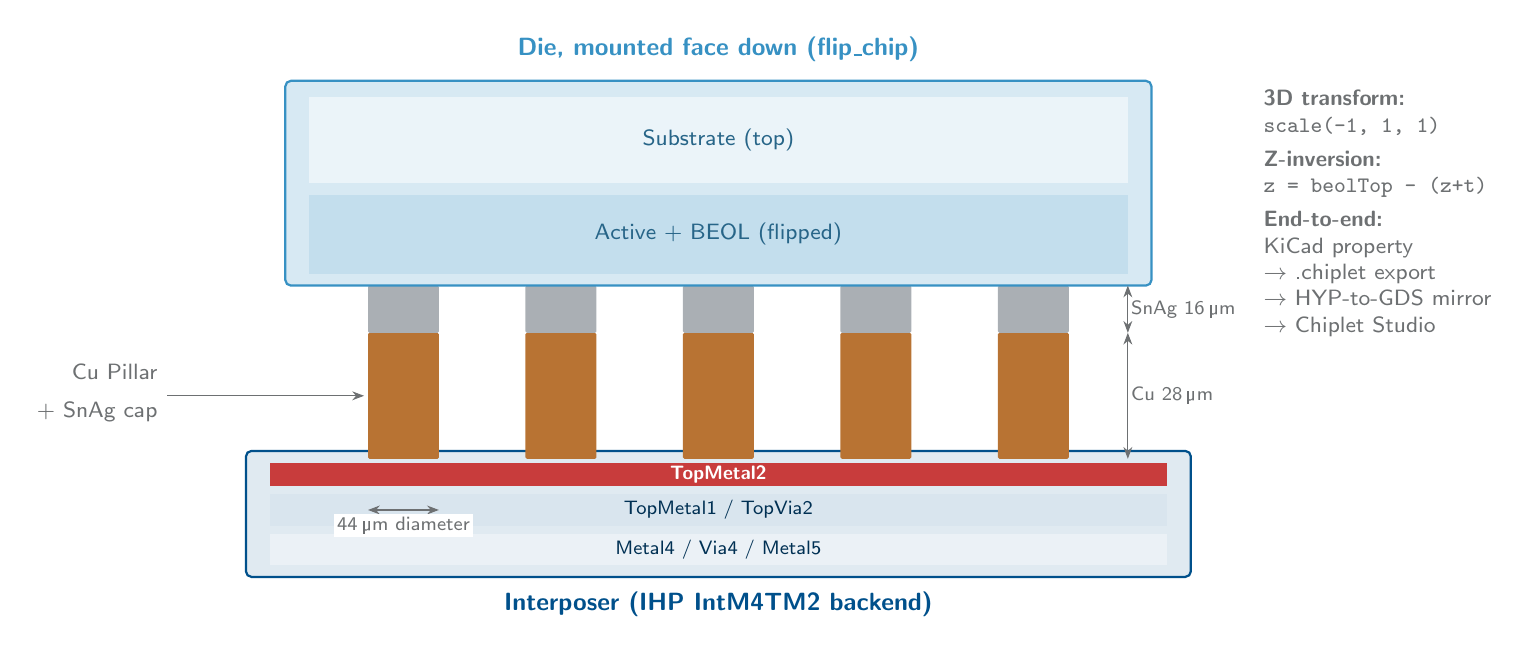
\begin{tikzpicture}[
    lbl/.style={font=\sffamily\small\bfseries, text=IHPfg},
    sublbl/.style={font=\sffamily\footnotesize, text=IHPaccent},
    codelbl/.style={font=\ttfamily\footnotesize, text=IHPaccent},
    dim/.style={
        {Stealth[length=1.5mm]}-{Stealth[length=1.5mm]},
        line width=0.4pt, color=IHPaccent
    },
    dimlbl/.style={font=\sffamily\scriptsize, text=IHPaccent, fill=white, inner sep=1pt}
]

% === INTERPOSER (bottom, wide) ===
\fill[cInterposer!12, draw=cInterposer, line width=0.8pt, rounded corners=2pt]
    (0, 0) rectangle (12, 1.6);

% Metal layers inside interposer (simplified)
\fill[cInterposer!8] (0.3, 0.15) rectangle (11.7, 0.55);
\node[font=\sffamily\scriptsize, text=cInterposer!60!black] at (6, 0.35) {Metal4 / Via4 / Metal5};
\fill[cInterposer!15] (0.3, 0.65) rectangle (11.7, 1.05);
\node[font=\sffamily\scriptsize, text=cInterposer!60!black] at (6, 0.85) {TopMetal1 / TopVia2};

% TopMetal2 pads
\fill[cTM2] (0.3, 1.15) rectangle (11.7, 1.45);
\node[font=\sffamily\scriptsize\bfseries, text=white] at (6, 1.30) {TopMetal2};

\node[lbl, text=cInterposer] at (6, -0.35) {Interposer (IHP IntM4TM2 backend)};

% === Cu-Pillar bumps (5 bumps) ===
\foreach \x in {2.0, 4.0, 6.0, 8.0, 10.0} {
    % Cu Pillar body
    \fill[cCuPillar, rounded corners=0.5pt] (\x-0.45, 1.50) rectangle (\x+0.45, 3.10);
    % SnAg cap
    \fill[cSnAg, rounded corners=0.5pt] (\x-0.45, 3.10) rectangle (\x+0.45, 3.70);
}

% === FLIPPED DIE (on top, face-down) ===
\fill[cDie!20, draw=cDie, line width=0.8pt, rounded corners=2pt]
    (0.5, 3.70) rectangle (11.5, 6.30);

% Layers inside die (flipped -- active at bottom, substrate at top)
\fill[cDie!30] (0.8, 3.85) rectangle (11.2, 4.85);
\node[font=\sffamily\footnotesize, text=cDie!70!black] at (6, 4.35) {Active + BEOL (flipped)};
\fill[cDie!10] (0.8, 5.00) rectangle (11.2, 6.10);
\node[font=\sffamily\footnotesize, text=cDie!70!black] at (6, 5.55) {Substrate (top)};

\node[lbl, text=cDie] at (6, 6.70) {Die, mounted face down (flip\_chip)};

% === Dimension labels ===
% Cu Pillar height
\draw[dim] (11.2, 1.50) -- (11.2, 3.10);
\node[dimlbl, right] at (11.2, 2.30) {Cu 28\,\textmu m};

% SnAg height
\draw[dim] (11.2, 3.10) -- (11.2, 3.70);
\node[dimlbl, right] at (11.2, 3.40) {SnAg 16\,\textmu m};

% Pillar diameter
\draw[dim] (2.0-0.45, 0.85) -- (2.0+0.45, 0.85);
\node[dimlbl, below] at (2.0, 0.80) {44\,\textmu m diameter};

% === Annotations (right side) ===
\node[font=\sffamily\footnotesize, text=IHPaccent, anchor=north west, align=left]
    at (12.8, 6.3) {
        \textbf{3D transform:}\\
        \texttt{scale(-1, 1, 1)}\\[1mm]
        \textbf{Z-inversion:}\\
        \texttt{z = beolTop - (z+t)}\\[1mm]
        \textbf{End-to-end:}\\
        KiCad property\\
        $\rightarrow$ .chiplet export\\
        $\rightarrow$ HYP-to-GDS mirror\\
        $\rightarrow$ Chiplet Studio
    };

% Cu-pillar label
\draw[IHPaccent, line width=0.4pt, -{Stealth[length=1.5mm]}]
    (-1.0, 2.30) -- (1.50, 2.30);
\node[sublbl, anchor=east] at (-1.0, 2.60) {Cu Pillar};
\node[sublbl, anchor=east] at (-1.0, 2.10) {+ SnAg cap};

\end{tikzpicture}
\end{document}
